\documentclass{article}
\usepackage[utf8]{inputenc}
\usepackage[spanish]{babel}
\usepackage{graphicx}
\graphicspath{ {images/} }

\begin{document}

\begin{titlepage}
    \begin{center}
        \vspace*{1cm}
            
        \Huge
        \textbf{Análisis e Informe}
            
        \vspace{0.5cm}
        \LARGE
        Parcial 2
            
        \vspace{1.5cm}
            
        \textbf{Danier Santiago Ortega Restrepo}\\
        \textbf{c.c.1036681098}\\
        \textbf{danier.ortega@udea.edu.co}
            
        \vfill
            
        \vspace{0.8cm}
            
        \Large
        Despartamento de Ingeniería Electrónica y Telecomunicaciones\\
        Universidad de Antioquia\\
        Medellín\\
       Septiembre de 2021
            
    \end{center}
\end{titlepage}

\newpage
\tableofcontents
\section{RECURSOS}
Despues de leer las indicaciones del parcial 2, primero se tendran en cuenta los recursos disponibles para la realizacion de este, se estudiaran conceptos de manejo de leds RGB(red green and blue), uso de la plataforma Tinkercad, arduino, lenguaje C++(Qt creator), manejo y libreria para el uso de tiras led neopixel, informacion multimedia relacionada con el proyecto y enfasis en el tiempo de realizacion.

Algunos recursos probables pero de analizar, circuito integrado, entorno de desarrollo arduino, ya sea online o descargar la app.

\section{PROPUESTA}
Una propuesta para empezar el parcial seria empezar por practicar con algunos leds RGB y practicar su funcionamiento y asi practicar su funcionamiendo y maniobrabilidad de colores a conveniencia del usuario.

Practicar el procesamiento de imagenes dictado por el profesor y buscar ayudas para la implementacion de esta parte fundamental, ya que a partir de el manejo adecuado de la imagen dependera la adaptacion a el arreglo de leds.

Crear funciones para lectura de imagen, adaptacion de imagen para el tamaño 8x8 sin importar la dimension de la imagen agregada, implementar una clase que trabaje con los pixeles que contega la imagen y retorne bits para implementarlos en la placa arduino y trasmitirlos a los leds 8x8.

Adaptar el codigo c++ trabajado en Qt al arduino y sus condiciones, ademas de tener en cuenta el tamaño de las variables para evitar lentitud en el procesamiento de los leds en tinkercad.

Leer archivos PNG en Qt, para esto se debe investigar como se trabaja la lectura y organizar estos datos de salida de tal forma que se puedan ingresar a la placa de arduino por las entradas seriales.

Crear la matriz de leds e implementar un metodo de organizacion de tal forma que se pueda trabajar con cada uno  de los leds de manera acertada, verificar metodos de submuestreo y muestreo para las imagenes, estudiar algoritmos de estos metodos ateriormente mencionados.

\begin{figure}
\section{IDEA}
En la imagen siguiente vemos una idea de partida para el parcial en donde se trabaja desde la parte en que se ingresan los datos a la placa de arduino en el entorno tikercad para su posterior funcionamiento.\\
    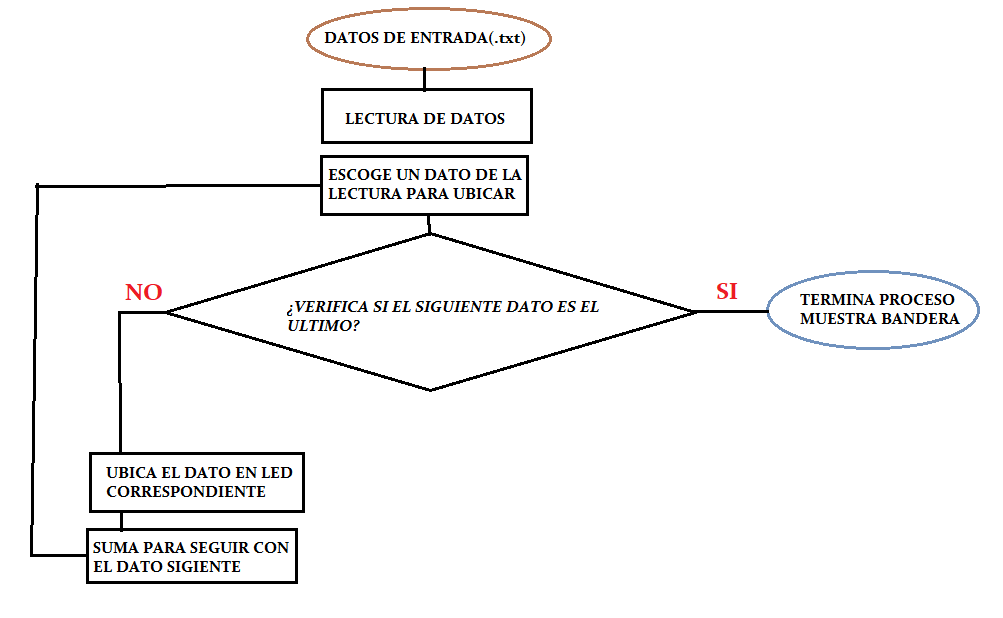
\includegraphics[width=10cm]{diagrama.png}
    \centering
    \caption{Diagrama de idea general}
    \label{fig:diagrama}
    \end{figure}

\begin{figure}
\section{IDEA DE TRABAJO DE IMAGENES}
Segun la guia explicada por el porfesor en la clase, primero hay que leer la imagen deseada, analizar los datos de dicha imagen como sus dimensiones, verificar los colores de cada uno de sus pixeles determinados como red,green y blue (rgb).

Luego de esto investigar o diseñar un algoritmo de submuestreo para adaptar la imagen a nuestro arreglo de tiras neopixel, en caso de que la imagen sea menor al arreglo realizar un muestreo para adaptar la imagen al arreglo para esto se deberan tener en cuenta algunos metodos de interpolacion de imagenes.\\
    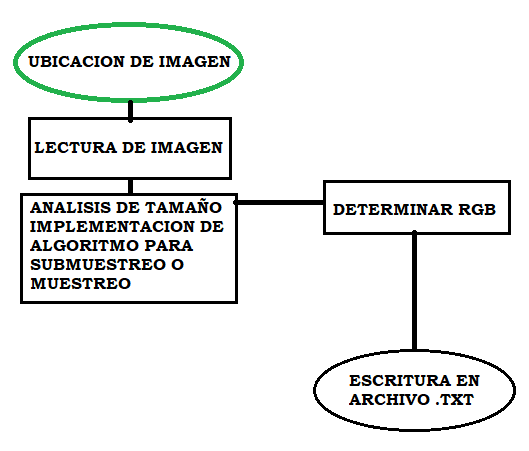
\includegraphics[width=10cm]{diagrama2.png}
    \centering
    \caption{Idea general(Qt c++)}
    \label{fig:diagrama2}
    \end{figure}

\begin{figure}   
\section{PROCESO TINKERCAD}
Se creo un arreglo de 8 tiras de neopixel, cada una de las tiras contiene 8 leds para un total de 64 leds, unidas por sus respectivas entradas y salidas, ademas se conectaron a una de las entradas seriales de la placa de arduino en el pin numero 2 por recomendacion de los profesores se agrego un suministro de energia con un paso de corriente de 20A.

    \includegraphics[width=10cm]{leds.png}
    \centering
    \caption{Orden de leds}
    \label{fig:leds}
    \end{figure}

\begin{figure}
\section{CODIGO ARDUINO}
Incialmente se escribio codigo en tinkercad de tal forma que al ingresar datos separados por coma se leyera en el codigo de arduino, se creo un arreglo de tamaño 192 porque cada uno de los datos ingresados llegarian en un orden de tres cada uno por los colores RGB, entonces ya que la cantidad de leds son 64 para cada led corresponde de a tres datos del arreglo, 3x64=192(tamaño del arreglo).
Ademas se condiciono para que en caso de que todos los valores de RGB fueran su maximo contenido de memoria o sea 255,255,255 al menos uno se le reducia el valor para que quedara en 254.

    \includegraphics[width=10cm]{code_arduino.png}
    \centering
    \caption{Codigo de arduino}
    \label{fig:code_arduino}
    \end{figure}
 
\begin{figure}   
\section {CODIGO QT}
En el incio se trabajo con las ayudas suministradas por los profesores para acceder al tamaño de las imagenes, luego se hizo pruebas con un cout para verificar el tamaño de algunas imagenes, despues se hizo pruebas con las ayudas brindadas para obtener la imformacion RGB que contenian los pixeles de la imagen leida.
A partir de lo anterior se empezo con la busqueda de algoritmo para la reduccion de una imagen a un conjunto de datos deseado, en este caso necesitabamos reducir el tamaño de una imagen (bandera de algun pais) a el tamaño de una matriz 8x8, se leyo codigo con la implementacion de interpolacion bilineal\cite{articulo_stackoverflow} en foro virtual.

    \includegraphics[width=8cm]{lectura_image.png}
    \centering
    \caption{Lectura de imagen}
    \label{fig:lectura_image}

\subsection{ARREGLOS}
Despues de analizar articulos, foros y archivos multimedia\cite{Subsampling}, se intento imprimir en la terminal desde Qt, una matriz del tamaño de cada imagen lo cual se volvio complicado de trabajar, despues se intento imprimir matrices con imagenes de tamaño pequeño o cercano a la matriz solicitada 8x8, para esto empezamos con con la impresion de uno de sus datos, por ejemplo de una matriz 15x15 se imprimio los datos de cada unos de sus pixeles en color Red, despues el color Green y respectivamente su color Blue.

Ademas al ser imagenes pequeñas se pudo ingresar estos datos RGB a un solo arreglo[n][m] tipo string, gracias a esto se pudo probar algunos arreglos separados por coma en el codigo ubicado en tinkercad.

\subsection{CICLOS}
Despues de analizar el comportamiento extrayendo imformacion de algunas imagenes de tamaño pequeño a traves de ciclos y condicionales guiados por su ancho y altura, se decidio cortar u omitir algunas filas y colunmas con la intencion de reducir su tamaño, se obtuvieron resultaron de reduccion pero ordenes incorrectos.
\end{figure}

\begin{figure} 
\subsection{RECORRIDO POR PASOS}
Se implemento un metodo en el cual se divide el ancho y la altura por el tamaño de la matriz o arreglo deseado en nuestro caso 8x8, al dividir el ancho entre 8 obtendremos un valor con el cual daremos pasos sobre el tamaño ariginal de la imagen sacando valores en cada paso sobre el eje X, de igual forma se divide la altura sobre 8, para despues dar pasos sobre el eje Y.
Se crean variables tipo long double para evitar perder distancias al dividir los tamaños por numeros enteros y asi tener pasos mas acertados sobre las imagenes de gran tamaño.

    \includegraphics[width=11cm]{reduccion.png}
    \centering
    \caption{Reduccion de imagen}
    \label{fig:reduccion}
    \end{figure}

\begin{figure} 
\section{ESCRITURA EN ARCHIVO DE TEXTO}
La parte de esritura sobre un archivo.txt se recopilo los conocimientos de practicas anteriores donde se debe tener en cuenta la verificacion de un archivo abierto y tener en cuenta que despues de modificarlo se debe cerrar.
Se creo un ciclo el cual escribia uno por uno los datos con sus respectivos RGB separados por una coma en un archivo llamado datos.txt.

    \includegraphics[width=11cm]{escritura.png}
    \centering
    \caption{Escritura en archivo.txt}
    \label{fig:escritura}
    \end{figure}
    
\begin{figure}
\subsection{datos.txt}
En la siguiente imagen se ve como quedan los datos en un archivo de texto listos para copiar y pegar en tinkercad.

    \includegraphics[width=11cm]{datos_txt.png}
    \centering
    \caption{datos.txt}
    \label{fig:datos_txt}
\end{figure}

\begin{figure} 

\section{EJEMPLO}
Aca tenemos un ejemplo de como funciona los datos en el entorno de tinkercad con la bandera de Mexico.

    \includegraphics[width=12cm]{ejemplo.png}
    \centering
    \caption{Ejemplo de bandera}
    \label{fig:ejemplo}
    \end{figure}

\begin{figure} 
\section{DIFICULTADES}
Los principales problemas que se tuvieron fueron el tiempo ya que por cuestiones laborales y academicas el tiempo se ve reducido, aunque los profes dieron buen plazo de entrega la presion por tiempo de las demas asignaturas generan un trabajo menos detallado y mas rapido.
Otro problema fue analizar que metodo se usaria para reducir la imagen, en el metodo que use, al trabajar con variables long double y no tomar valores enteros, hace que el programa responda a las imagenes pequeñas tambien, aunque no de manera muy acertada.
\end{figure}

\begin{figure} 
\section{CONCLUSION}
Este trabajo me trajo conocimientos muy importantes sobre como funcionan las imagenes digitales, la relacion entre los colores RGB en cada pixel son de valor absoluto, ademas me genero un mapa el cual no conocia sobre los diferentes metodos que se usan en muchas plataformas para procesar y manejar las imagenes.
\end{figure}

\begin{figure}  
\bibliographystyle{IEEEtran}
\bibliography{references}
\end{figure}  
\end{document}
